\chapter{Química organometálica: enlace y ligandos}\label{ch:b3:organometallic-bonding}

En 1951, dos grupos de investigación obtuvieron, de forma independiente, un polvo naranja,
estable al aire, de fórmula $\ce{FeC10H10}$ que no tenía sentido: el hierro no suele formar
enlaces estables con el carbono, y menos aún con dos anillos ciclopentadienilo a
la vez. En menos de un año se estableció su estructura: el hierro se sitúa entre dos
anillos paralelos, unido por igual a los diez átomos de carbono, en un sándwich. El ferroceno
abrió la química organometálica moderna, cuyos catalizadores fabrican hoy la mayor parte de los
polímeros, fármacos y productos de química fina del mundo (\cref{ch:b3:homogeneous-catalysis}).
Este capítulo explica cómo se enlazan los metales al monóxido de carbono, a las fosfinas, a los alquenos,
a los anillos, a los \omterm{def:b3:organometallic-bonding:carbene}{carbenos} y entre sí, y cómo la \omterm{def:b3:organometallic-bonding:isolobal}{analogía isolobular} conecta
los fragmentos organometálicos con la química orgánica del carbono.

\begin{recall}
El volumen del primer año definió los compuestos organometálicos y usó los reactivos de Grignard.
El volumen del segundo año introdujo la regla de los 18 electrones y el recuento de electrones de valencia,
la hapticidad, los ligandos $\pi$-aceptores y $\pi$-dadores con la retrodonación, las etapas
elementales de las reacciones organometálicas (adición oxidante, eliminación reductora,
inserción) y los orbitales de fragmento. El \cref{ch:b3:group-theory-applied} contó
las tensiones CO \omterm{def:b3:group-theory-applied:activity}{activas en IR} de los carbonilos y construyó combinaciones adaptadas a la
simetría; el \cref{ch:b3:complex-spectra-magnetism} relacionó los momentos magnéticos
con los electrones desapareados.
\end{recall}

\begin{omfigure}
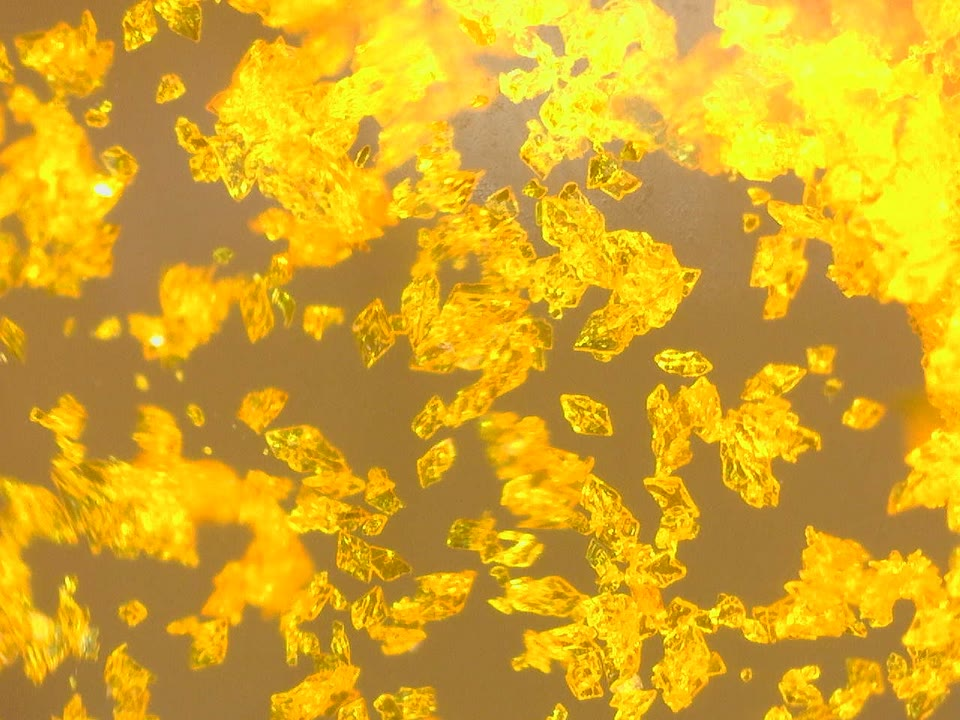
\includegraphics[width=0.5\linewidth]{images/book4/ferrocene-crystals.jpg}

{\small Cristales de ferroceno, $\ce{Fe(C5H5)2}$: un compuesto organometálico naranja,
estable al aire, que sublima al calentarlo suavemente.}
\end{omfigure}

\section{Recuento de electrones y estados de oxidación}

\begin{method}[Contar electrones de dos maneras]\label{met:b3:organometallic-bonding:count}
\begin{enumerate}
  \item Método de los ligandos neutros (covalente): el metal aporta tantos electrones como su número
        de grupo; cada ligando, tomado neutro, aporta 1 (H, \ce{CH3}, Cl, el
        $\eta^1$-alilo), 2 (CO, \ce{PR3}, alqueno) o más ($\eta^5$-\ce{C5H5} 5, $\eta^6$-\ce{C6H6} 6); se suma uno por cada
        enlace metal--metal y se corrige según la carga global.
  \item Método iónico: ligandos como H, \ce{CH3}, Cl, \ce{C5H5} se cuentan como aniones (2, 2,
        2 y 6 electrones), y el metal, como el catión $d^n$ resultante; los ligandos neutros,
        como antes.
  \item Ambos dan el mismo total; el método iónico da además el estado de oxidación
        y el número $d^n$.
\end{enumerate}
\end{method}

\begin{example}[Recuento]\label{ex:b3:organometallic-bonding:count}
$\ce{Fe(CO)5}$: $8 + 5 \times 2 = 18$, hierro(0), $d^8$. Ferroceno: método neutro, $8 + 2 \times 5 = 18$; método iónico,
$\ce{Fe^{2+}}$ ($d^6$, 6) $+ 2 \times 6$ ($\ce{C5H5-}$) $= 18$, hierro(II). $\ce{Mn2(CO)10}$: cada Mn, $7 + 5 \times 2 + 1$ (el enlace
Mn--Mn) $= 18$. Los complejos plano-cuadrados $d^8$ como $\ce{[PtCl4]^{2-}}$ o el catalizador de Wilkinson
$\ce{RhCl(PPh3)3}$ tienen 16 electrones: su orbital vacío de tipo $p_z$ está demasiado alto para llenarse, y
los complejos plano-cuadrados de 16 electrones son tan estables como los de 18.
\end{example}

\section{Carbonilos y fosfinas}

\begin{definition}[Carbonilos metálicos]\label{def:b3:organometallic-bonding:carbonyl}
Un \emph{carbonilo metálico}\index{carbonilo metalico@carbonilo metálico} es un complejo con ligandos
monóxido de carbono. Un \emph{carbonilo terminal}\index{carbonilo terminal} está unido a un solo
metal a través del carbono; un \emph{carbonilo puente}\index{carbonilo puente} tiende un puente entre
dos (o tres) metales.
\end{definition}

Ludwig Mond descubrió en 1890 que el níquel reacciona con el monóxido de carbono a temperatura
ordinaria para dar el líquido volátil $\ce{Ni(CO)4}$, que al calentarlo se descompone de nuevo en
níquel puro: la base de un proceso de refino. El monóxido de carbono se une a
los metales de transición a través de su orbital ocupado más alto, un par solitario $\sigma$ situado sobre todo
en el carbono, y acepta electrones en sus orbitales $\pi^*$ vacíos, también mayores en el
carbono.

\begin{definition}[Enlace sinérgico]\label{def:b3:organometallic-bonding:synergic}
El \emph{enlace sinérgico}\index{enlace sinergico@enlace sinérgico} es el refuerzo mutuo de la
donación $\sigma$ de un ligando a un metal y de la retrodonación $\pi$ del metal al
ligando: la donación enriquece al metal en electrones y lo hace más dispuesto a
devolverlos, y la retrodonación alivia la carga acumulada por la donación.
\end{definition}

\begin{omfigure}
\begin{tikzpicture}[font=\small, >=Stealth]
  % sigma donation
  \fill[black!70] (0,0) circle (0.14); \node[anchor=north] at (0,-0.4) {M};
  \pic at (0,0) {omlobe={-0.7}{180}};
  \pic at (0,0) {omlobe={0.9}{0}};
  \node[circle, fill=black!40, inner sep=1.6pt] at (1.9,0) {};
  \node[circle, fill=omThm!70, inner sep=1.6pt] at (3.0,0) {};
  \pic at (1.9,0) {omlobe={0.85}{180}};
  \node[font=\scriptsize, anchor=north] at (1.9,-0.25) {C};
  \node[font=\scriptsize, anchor=north] at (3.0,-0.25) {O};
  \draw[->, thick, omThm] (1.4,0.55) to[bend right=30] (0.6,0.55);
  \node[anchor=north] at (1.5,-1.55) {donación $\sigma$};
  % pi back-donation
  \begin{scope}[xshift=6.0cm]
    \fill[black!70] (0,0) circle (0.14); \node[anchor=north] at (0,-1.1) {M};
    \pic at (0,0) {omdxz};
    \node[circle, fill=black!40, inner sep=1.6pt] at (1.9,0) {};
    \node[circle, fill=omThm!70, inner sep=1.6pt] at (3.0,0) {};
    \pic at (1.9,0) {omp={0.9}{90}};
    \pic at (3.0,0) {omp={-0.6}{90}};
    \draw[->, thick, omThm] (0.6,1.05) to[bend left=30] (1.6,1.05);
    \node[anchor=north] at (1.5,-1.55) {retrodonación $\pi$};
  \end{scope}
\end{tikzpicture}

{\small \omterm{def:b3:organometallic-bonding:synergic}{Enlace sinérgico} del monóxido de carbono. Izquierda: el par solitario del carbono (orbital
$\sigma$) dona hacia un orbital metálico vacío de tipo $\sigma$. Derecha: un orbital $d$ lleno del metal
($d_{xz}$, con sus dos ejes) se solapa con el orbital $\pi^*$ vacío del CO, mayor en el
carbono, cuyos lóbulos coinciden con sus fases: los electrones refluyen hacia un orbital que es
antienlazante entre C y O.}
\end{omfigure}

\begin{proposition}[Frecuencias de tensión del CO]\label{prop:b3:organometallic-bonding:co-frequency}
Cuanto más retrodona un metal hacia los orbitales $\pi^*$ de un ligando CO, menor es el
número de onda de tensión C--O.
\end{proposition}

\begin{proof}[Argumento]
Los orbitales $\pi^*$ del CO son antienlazantes entre C y O: poblarlos debilita el
enlace C--O y reduce su \omterm{def:b3:quantum-model-systems:oscillator}{constante de fuerza}, y por tanto el número de onda de tensión, que
varía como la raíz cuadrada de la \omterm{def:b3:quantum-model-systems:oscillator}{constante de fuerza} (\cref{ch:b3:rovibrational-spectroscopy}).
La donación $\sigma$ retira electrones de un orbital casi no enlazante (ligeramente
antienlazante) para C--O, lo que por sí solo elevaría un poco el número de onda: la
disminución observada muestra que domina la retrodonación.
\end{proof}

El monóxido de carbono libre tiene su fundamental en $\omega_e - 2\omega_ex_e = \qty{2143}{cm^{-1}}$; los \omterm{def:b3:organometallic-bonding:carbonyl}{carbonilos
terminales} de los complejos neutros absorben aproximadamente entre 1900 y \qty{2100}{cm^{-1}},
y los \omterm{def:b3:organometallic-bonding:carbonyl}{carbonilos puente}, más abajo aún. A lo largo de una serie isoelectrónica, un carbonilo
aniónico absorbe a un número de onda menor que el neutro, y uno catiónico, a uno
mayor: cuanto más rico en electrones es el metal, más retrodona. El número de
bandas, por la simetría (\cref{ch:b3:group-theory-applied}), da la geometría.
% ledger: diat:CO.we, diat:CO.wexe

\begin{proposition}[Interacciones $\pi$ y desdoblamiento del campo de ligandos]\label{prop:b3:organometallic-bonding:pi-delta}
En un complejo octaédrico, los ligandos $\pi$-aceptores aumentan $\Delta_{\mathrm o}$, y los ligandos $\pi$-dadores
lo disminuyen.
\end{proposition}

\begin{proof}
Los orbitales $e_g$ solo tienen simetría $\sigma$. Los orbitales $t_{2g}$ ($d_{xy}$, $d_{xz}$, $d_{yz}$) coinciden con una combinación $t_{2g}$
de orbitales $\pi$ de los ligandos: para $d_{xy}$, los cuatro ligandos del plano $xy$
ofrecen cada uno un orbital $\pi$ perpendicular a su eje M--L dentro de ese plano, y la
combinación de signos alternos tiene la simetría de $d_{xy}$ (las demás
combinaciones se transforman como $t_{1g}$, $t_{1u}$ y $t_{2u}$ y no encuentran pareja $d$). Dos orbitales de
la misma simetría se mezclan y se repelen: el inferior baja y el superior sube. Un
$\pi$-aceptor ofrece orbitales vacíos por encima del conjunto $t_{2g}$, que baja: $\Delta_{\mathrm o}$
aumenta. Un $\pi$-dador ofrece orbitales llenos por debajo de él, que lo empujan hacia arriba: $\Delta_{\mathrm o}$
disminuye. El nivel $e_g$ no se ve afectado en ninguno de los dos casos.
\end{proof}

Por eso el CO y el \ce{CN-} se sitúan en el extremo fuerte de la serie espectroquímica, y
los haluros y el hidróxido en el extremo débil, como indicó el volumen del segundo año.

\begin{definition}[Parámetros de Tolman]\label{def:b3:organometallic-bonding:tolman}
El \emph{ángulo cónico de Tolman}\index{angulo conico de Tolman@ángulo cónico de Tolman} de una fosfina es el ángulo
en el vértice del cono, centrado en el metal a una distancia estándar, que encierra justo
las superficies de van der Waals de sus sustituyentes: una medida de su tamaño.
El \emph{parámetro electrónico de Tolman}\index{parametro electronico de Tolman@parámetro electrónico de Tolman} es el
número de onda de la tensión CO simétrica del $\ce{Ni(CO)3L}$: cuanto más fuertemente
dona la fosfina L, menor es.
\end{definition}

Las fosfinas se ajustan de forma independiente en tamaño y en donación electrónica mediante sus
sustituyentes: las trialquilfosfinas son dadores más fuertes que las triarilfosfinas, y
los fosfitos, los más débiles; la $\ce{P(tBu)3}$ es mucho más voluminosa que la $\ce{PMe3}$. Las fosfinas voluminosas favorecen
los números de coordinación bajos y la disociación rápida de ligandos, y por eso
aparecen en tantos catalizadores.

\section{Ligandos $\pi$}

\begin{definition}[Modelo de Dewar--Chatt--Duncanson]\label{def:b3:organometallic-bonding:dcd}
El \emph{modelo de Dewar--Chatt--Duncanson}\index{modelo de Dewar--Chatt--Duncanson} del
enlace de un alqueno con un metal combina la donación $\sigma$ desde el orbital $\pi$ C=C
hacia un orbital metálico vacío con la retrodonación desde un orbital $d$ lleno del metal hacia
el orbital $\pi^*$ C=C. Su límite de retrodonación fuerte es un
\emph{metalaciclopropano}\index{metalaciclopropano}, un anillo de tres miembros
con dos enlaces $\sigma$ M--C y un enlace sencillo C--C.
\end{definition}

\begin{proposition}[Consecuencias de la retrodonación hacia un alqueno]\label{prop:b3:organometallic-bonding:dcd}
La coordinación alarga el enlace C=C y dobla los sustituyentes hacia atrás, alejándolos
del metal, tanto más cuanto mayor es la retrodonación.
\end{proposition}

\begin{proof}[Argumento]
Retirar electrones del orbital $\pi$ (enlazante) y añadirlos al orbital $\pi^*$
(antienlazante) rebajan ambos el orden de enlace C--C. La mezcla de carácter $\pi^*$
rehibrida los carbonos hacia $sp^3$, cuyos enlaces con los sustituyentes apuntan lejos
del metal, hacia la geometría del \omterm{def:b3:organometallic-bonding:dcd}{metalaciclopropano}.
\end{proof}

\begin{omfigure}
\begin{tikzpicture}[font=\small, >=Stealth]
  \fill[black!70] (0,0) circle (0.14); \node[anchor=north] at (0,-1.1) {M};
  \pic at (0,0) {omlobe={0.9}{0}};
  \foreach \y in {0.45,-0.45}{\node[circle, fill=black!40, inner sep=1.6pt] at (1.9,\y) {};}
  \pic at (1.9,0.45) {omp={-0.75}{0}};
  \pic at (1.9,-0.45) {omp={-0.75}{0}};
  \draw[->, thick, omThm] (1.3,1.0) to[bend right=30] (0.5,0.6);
  \node[anchor=north] at (1.2,-1.4) {$\sigma$: $\pi$(C=C) $\to$ M};
  \begin{scope}[xshift=5.6cm]
    \fill[black!70] (0,0) circle (0.14); \node[anchor=north] at (0,-1.1) {M};
    \pic at (0,0) {omdxy};
    \foreach \y in {0.45,-0.45}{\node[circle, fill=black!40, inner sep=1.6pt] at (1.9,\y) {};}
    \pic at (1.9,0.45) {omp={-0.75}{0}};
    \pic at (1.9,-0.45) {omp={0.75}{0}};
    \draw[->, thick, omThm] (0.7,0.9) to[bend left=30] (1.5,0.9);
    \node[anchor=north] at (1.2,-1.4) {$\pi$: M $\to$ $\pi^*$(C=C)};
  \end{scope}
\end{tikzpicture}

{\small El \omterm{def:b3:organometallic-bonding:dcd}{modelo de Dewar--Chatt--Duncanson} de un alqueno unido lateralmente (C=C
vertical, el metal a la izquierda). Izquierda: el orbital $\pi$ lleno (dos orbitales $p$ en
fase) dona hacia un orbital metálico vacío. Derecha: un orbital $d$ lleno del metal
de fases coincidentes dona hacia el orbital $\pi^*$ vacío (los dos orbitales $p$ en oposición de
fase).}
\end{omfigure}

La sal de Zeise, $\ce{K[PtCl3(C2H4)]}$, preparada en 1827, fue el primer compuesto organometálico
de un metal de transición; su eteno es perpendicular al plano \ce{PtCl3}, como
predice el modelo. El alilo ($\eta^3$), los dienos ($\eta^4$), los arenos ($\eta^6$) y el anillo
ciclopentadienilo ($\eta^5$) se unen del mismo modo a través de varios carbonos a la vez.

\begin{definition}[Metalocenos]\label{def:b3:organometallic-bonding:metallocene}
Un \emph{compuesto sándwich}\index{compuesto sandwich@compuesto sándwich} tiene un metal entre dos
ligandos anulares planos y paralelos unidos a través de todos sus carbonos; un
\emph{metaloceno}\index{metaloceno} es un compuesto sándwich con dos anillos
$\eta^5$-ciclopentadienilo, $\ce{M(C5H5)2}$.
\end{definition}

\begin{proposition}[Los orbitales frontera del ferroceno]\label{prop:b3:organometallic-bonding:ferrocene}
En un \omterm{def:b3:organometallic-bonding:metallocene}{metaloceno} de anillos paralelos ($D_{5d}$), los orbitales $d$ del metal se desdoblan en $e_{2g}$
($d_{xy}$, $d_{x^2-y^2}$) y $a_{1g}$ ($d_{z^2}$), casi no enlazantes y próximos entre sí, y $e_{1g}^\ast$ ($d_{xz}$,
$d_{yz}$), fuertemente antienlazantes; el ferroceno, con seis electrones $d$ en $e_{2g}^4a_{1g}^2$, tiene 18
electrones y ningún electrón desapareado.
\end{proposition}

\begin{proof}[Argumento]
Los orbitales $\pi$ de los dos anillos se combinan en pares adaptados a la simetría $a_{1g}$, $a_{2u}$,
$e_{1g}$, $e_{1u}$, $e_{2g}$, $e_{2u}$ (a partir de los cinco orbitales $\pi$ de cada anillo, con cero, uno y dos
planos nodales que contienen el eje). La combinación $e_{1g}$ llena de los anillos se solapa
fuertemente con $d_{xz}$, $d_{yz}$ (un plano nodal que contiene el eje cada uno): forman orbitales
enlazantes, sobre todo de los anillos, y antienlazantes $e_{1g}^\ast$, sobre todo del metal, empujados muy arriba. $d_{xy}$, $d_{x^2-y^2}$
(dos planos nodales) solo encuentran los orbitales $e_{2g}$ vacíos de los anillos y se estabilizan
ligeramente por retrodonación; $d_{z^2}$ apunta al hueco del centro de cada anillo y
apenas se solapa. Seis electrones llenan $e_{2g}$ y $a_{1g}$; con los doce electrones de las
combinaciones enlazantes de los anillos, el recuento es 18.
\end{proof}

\begin{omfigure}
\begin{tikzpicture}[font=\small]
  % sandwich drawing
  \begin{scope}[xshift=-1.0cm]
    \draw[thick, fill=black!8] (0,1.0) ellipse (1.0 and 0.3);
    \draw[thick, fill=black!8] (0,-1.0) ellipse (1.0 and 0.3);
    \foreach \a in {90,162,234,306,18}{\fill[black!60] ({cos(\a)},{1.0+0.3*sin(\a)}) circle (0.07);
      \fill[black!60] ({cos(\a)},{-1.0+0.3*sin(\a)}) circle (0.07);}
    \shade[ball color=orange!70!brown] (0,0) circle (0.2);
    \node[anchor=west] at (0.25,0) {Fe};
  \end{scope}
  % level diagram for four metallocenes
  \pic[transform shape] at (2.1,-0.9) {omlevel={u}{0.5}};
  \pic[transform shape] at (2.7,-0.9) {omlevel={ud}{0.5}};
  \pic[transform shape] at (2.4,-0.4) {omlevel={ud}{0.5}};
  \pic[transform shape] at (2.1,1.0) {omlevel={}{0.5}};
  \pic[transform shape] at (2.7,1.0) {omlevel={}{0.5}};
  \node[anchor=north] at (2.4,-1.3) {\ce{[FeCp2]+}};
  \node[anchor=north, font=\scriptsize] at (2.4,-1.75) {17 e$^-$};
  \pic[transform shape] at (4.3,-0.9) {omlevel={ud}{0.5}};
  \pic[transform shape] at (4.9,-0.9) {omlevel={ud}{0.5}};
  \pic[transform shape] at (4.6,-0.4) {omlevel={ud}{0.5}};
  \pic[transform shape] at (4.3,1.0) {omlevel={}{0.5}};
  \pic[transform shape] at (4.9,1.0) {omlevel={}{0.5}};
  \node[anchor=north] at (4.6,-1.3) {\ce{FeCp2}};
  \node[anchor=north, font=\scriptsize] at (4.6,-1.75) {18 e$^-$};
  \pic[transform shape] at (6.5,-0.9) {omlevel={ud}{0.5}};
  \pic[transform shape] at (7.1,-0.9) {omlevel={ud}{0.5}};
  \pic[transform shape] at (6.8,-0.4) {omlevel={ud}{0.5}};
  \pic[transform shape] at (6.5,1.0) {omlevel={u}{0.5}};
  \pic[transform shape] at (7.1,1.0) {omlevel={}{0.5}};
  \node[anchor=north] at (6.8,-1.3) {\ce{CoCp2}};
  \node[anchor=north, font=\scriptsize] at (6.8,-1.75) {19 e$^-$};
  \pic[transform shape] at (8.7,-0.9) {omlevel={ud}{0.5}};
  \pic[transform shape] at (9.3,-0.9) {omlevel={ud}{0.5}};
  \pic[transform shape] at (9.0,-0.4) {omlevel={ud}{0.5}};
  \pic[transform shape] at (8.7,1.0) {omlevel={u}{0.5}};
  \pic[transform shape] at (9.3,1.0) {omlevel={u}{0.5}};
  \node[anchor=north] at (9.0,-1.3) {\ce{NiCp2}};
  \node[anchor=north, font=\scriptsize] at (9.0,-1.75) {20 e$^-$};
  \node[anchor=east, font=\scriptsize] at (1.8,-0.9) {$e_{2g}$};
  \node[anchor=east, font=\scriptsize] at (1.8,-0.4) {$a_{1g}$};
  \node[anchor=east, font=\scriptsize] at (1.8,1.0) {$e_{1g}^\ast$};
\end{tikzpicture}

{\small Izquierda: la estructura en sándwich del ferroceno (anillos eclipsados). Derecha: los
orbitales frontera de base $d$ de los \omterm{def:b3:organometallic-bonding:metallocene}{metalocenos}, $e_{2g}$ y $a_{1g}$ casi no enlazantes, $e_{1g}^\ast$
antienlazante, llenos para el catión ferrocinio (17 electrones), el ferroceno (18),
el cobaltoceno (19) y el niqueloceno (20, un electrón en cada orbital $e_{1g}^\ast$, con los espines
paralelos por la regla de Hund).}
\end{omfigure}

\section{Carbenos, carbinos y enlaces metal--metal}

\begin{definition}[Carbenos y complejos carbénicos]\label{def:b3:organometallic-bonding:carbene}
Un \emph{carbeno}\index{carbeno} es una especie neutra $\ce{R2C}$ con un carbono divalente
que lleva dos electrones no enlazantes. Un \emph{complejo carbénico}\index{complejo carbenico@complejo carbénico}
tiene un ligando $\ce{CR2}$ unido a un metal por un doble enlace, $\ce{M=CR2}$. Un complejo de
\emph{carbeno de Fischer}\index{carbeno de Fischer} tiene un sustituyente heteroatómico
en el carbono carbénico y un metal de valencia baja con ligandos $\pi$-aceptores; su carbono
carbénico es electrófilo. Un complejo de \emph{carbeno de Schrock}\index{carbeno de Schrock} (alquilideno)
solo tiene sustituyentes C o H y un metal temprano de valencia alta; su carbono es
nucleófilo. Un \emph{carbeno N-heterocíclico}\index{carbeno N-heterociclico@carbeno N-heterocíclico} es un
carbeno cíclico flanqueado por dos átomos de nitrógeno, estable como compuesto libre y ligando
$\sigma$-dador fuerte.
\end{definition}

Los dos tipos de \omterm{def:b3:organometallic-bonding:carbene}{complejos carbénicos} difieren en la forma en que se comparte el enlace M=C.
En un \omterm{def:b3:organometallic-bonding:carbene}{carbeno de Fischer}, un \omterm{def:b3:organometallic-bonding:carbene}{carbeno} singlete dona su par solitario al metal y
recibe retrodonación en su orbital $p$ vacío, que el par solitario del heteroátomo
estabiliza también: el carbono sigue siendo pobre en electrones y lo atacan los nucleófilos. En un
\omterm{def:b3:organometallic-bonding:carbene}{carbeno de Schrock}, dos fragmentos triplete, el metal y el \omterm{def:b3:organometallic-bonding:carbene}{carbeno}, forman un enlace covalente $\sigma +
\pi$, polarizado hacia el carbono: el alquilideno se comporta como un iluro de Wittig.

\begin{definition}[Complejo de carbino]\label{def:b3:organometallic-bonding:carbyne}
Un \emph{complejo de carbino}\index{complejo de carbino} tiene un triple enlace entre un metal
y un carbono que lleva un sustituyente, $\ce{M#CR}$.
\end{definition}

\begin{definition}[Enlace $\delta$, enlace cuádruple]\label{def:b3:organometallic-bonding:delta}
Un \emph{enlace $\delta$}\index{enlace delta@enlace $\delta$} es un enlace cuyo orbital tiene dos planos nodales
que contienen el eje internuclear, formado por el solapamiento cara a cara de dos orbitales
$d$, como $d_{xy}$ y $d_{xy}$. Un \emph{enlace cuádruple}\index{enlace cuadruple@enlace cuádruple}
combina un enlace $\sigma$, dos $\pi$ y uno $\delta$ entre dos átomos metálicos.
\end{definition}

\begin{proposition}[{El \omterm{def:b3:organometallic-bonding:delta}{enlace cuádruple} del $[\mathrm{Re_2Cl_8}]^{2-}$}]\label{prop:b3:organometallic-bonding:quadruple}
En el $\ce{[Re2Cl8]^{2-}}$ (dos \ce{Re^{III}}, $d^4$ cada uno), los ocho electrones $d$ ocupan $\sigma^2\pi^4\delta^2$: un orden
de enlace de 4, que exige la disposición eclipsada de las dos unidades \ce{ReCl4}.
\end{proposition}

\begin{proof}
Con $z$ según el eje Re--Re y los átomos de Cl según $\pm x$ y $\pm y$ en cada Re, $d_{x^2-y^2}$
apunta hacia los cloruros y se usa en el enlace Re--Cl. Los otros cuatro orbitales $d$
de cada metal se solapan por pares: $d_{z^2}$ con $d_{z^2}$ a lo largo del eje ($\sigma$), $d_{xz}$ con $d_{xz}$ y $d_{yz}$
con $d_{yz}$ lateralmente ($\pi$, dos veces), $d_{xy}$ con $d_{xy}$ cara a cara ($\delta$, el más débil).
Ocho electrones llenan las cuatro combinaciones enlazantes. Girar una unidad $45^\circ$
alrededor de $z$ convierte su $d_{xy}$ en $d_{x^2-y^2}$, cuyo solapamiento con el otro $d_{xy}$ es nulo por
simetría: el enlace $\delta$, y con él la preferencia por la forma eclipsada, se pierde. Los
otros tres solapamientos tienen simetría cilíndrica o no cambian de magnitud.
\end{proof}

% ledger: geom:Re2Cl8.ReRe
La distancia Re--Re de \qty{2.24}{\angstrom} en la sal de potasio es muy corta para dos átomos metálicos, y los cloruros de las dos mitades están en efecto eclipsados, a pesar de
su repulsión estérica: el enlace $\delta$, por débil que sea, los mantiene así.

\begin{omfigure}
\tdplotsetmaincoords{58}{25}
\begin{tikzpicture}[tdplot_main_coords, font=\small, scale=1.15]
  \draw[thick, black!60] (0,0,0) -- (0,0,2.0);
  \foreach \z in {0,2.0}{
    \foreach \b in {0,90,180,270}{
      \draw[black!45] (0,0,\z) -- ({1.55*cos(\b)},{1.55*sin(\b)},\z);}
    \foreach \a/\s in {45/omphasepos, 135/omphaseneg, 225/omphasepos, 315/omphaseneg}{
      \path[\s, opacity=0.9] plot[domain=0:360, samples=48, smooth cycle]
        ({0.62*cos(\a)+0.55*cos(\x)*cos(\a)-0.26*sin(\x)*sin(\a)},
         {0.62*sin(\a)+0.55*cos(\x)*sin(\a)+0.26*sin(\x)*cos(\a)}, {\z});}
    \foreach \b in {0,90,180,270}{
      \node[circle, fill=green!45!black, inner sep=1.8pt] at ({1.55*cos(\b)},{1.55*sin(\b)},\z) {};}
    \shade[ball color=black!40] (0,0,\z) circle (0.14);}
  \node[anchor=east, xshift=-1.9cm] at (0,0,2.0) {Re};
  \node[anchor=east, xshift=-1.9cm] at (0,0,0) {Re};
\end{tikzpicture}

{\small La componente $\delta$ del \omterm{def:b3:organometallic-bonding:delta}{enlace cuádruple} del $\ce{[Re2Cl8]^{2-}}$: los orbitales $d_{xy}$ de
los dos átomos de renio (cuatro lóbulos cada uno, signos en azul y naranja) se enfrentan
a través del eje Re--Re, lóbulo sobre lóbulo del mismo signo. Los cloruros (en verde),
eclipsados, se sitúan según $x$ e $y$, entre los lóbulos.}
\end{omfigure}

\section{La analogía isolobular}

\begin{definition}[Fragmentos isolobulares]\label{def:b3:organometallic-bonding:isolobal}
Dos fragmentos moleculares son \emph{isolobulares}\index{fragmentos isolobulares} cuando el
número, la simetría, la energía aproximada y la forma de sus orbitales frontera, y el
número de electrones que contienen, son parecidos. La \emph{analogía
isolobular}\index{analogia isolobular@analogía isolobular} predice que los fragmentos isolobulares pueden sustituirse
unos a otros en las moléculas.
\end{definition}

\begin{proposition}[Series isolobulares]\label{prop:b3:organometallic-bonding:isolobal}
$\ce{CH3}$, $\ce{Mn(CO)5}$ y $\ce{CpFe(CO)2}$ son \omterm{def:b3:organometallic-bonding:isolobal}{isolobulares} (un orbital frontera, un electrón);
$\ce{CH2}$ y $\ce{Fe(CO)4}$ (dos orbitales, dos electrones); $\ce{CH}$ y $\ce{Co(CO)3}$ (tres orbitales,
tres electrones).
\end{proposition}

\begin{proof}[Argumento]
El $\ce{CH3}$ es un fragmento tetraédrico al que le falta un enlace: un orbital de tipo $sp^3$ con un
electrón, a uno del octeto. El $\ce{Mn(CO)5}$ es un octaedro al que le falta un ligando: la
posición vacía alberga un orbital híbrido que apunta hacia fuera; con $7 + 10 = 17$ electrones, está a uno
de 18, y su único electrón ocupa ese híbrido. Quitar dos o tres
ligandos (o enlaces) da dos o tres de esos orbitales y electrones, con el
mismo recuento en ambos lados: el $\ce{Fe(CO)4}$ tiene 16 electrones ($8 + 8$), a dos de 18;
el $\ce{Co(CO)3}$ tiene 15 ($9 + 6$), a tres.
\end{proof}

\begin{method}[Predecir una estructura por sustitución isolobular]\label{met:b3:organometallic-bonding:isolobal}
\begin{enumerate}
  \item Dividir el compuesto en fragmentos y contar los orbitales frontera
        y los electrones de cada uno.
  \item Sustituir cada fragmento por su pareja isolobular orgánica.
  \item El análogo orgánico, si existe, sugiere el enlace y la forma:
        el $\ce{Mn2(CO)10}$ es ``etano'', y el $\ce{Co3(CO)9CH}$ es ``tetraedrano'', $\ce{(CH)4}$, con tres CH
        sustituidos por $\ce{Co(CO)3}$.
\end{enumerate}
\end{method}

\begin{omfigure}
\begin{tikzpicture}[font=\small]
  \foreach \y/\l/\r/\n in {0/{\ce{CH3}}/{\ce{Mn(CO)5}}/1, -1.6/{\ce{CH2}}/{\ce{Fe(CO)4}}/2, -3.2/{\ce{CH}}/{\ce{Co(CO)3}}/3}{
    \node at (0,\y) {\l};
    \node at (5.2,\y) {\r};
    \node[font=\large] at (2.6,\y) {$\longleftrightarrow$};
    \node[font=\scriptsize, anchor=south] at (2.6,\y+0.15) {isolobulares};
    \node[font=\scriptsize, anchor=west] at (7.0,\y) {\ifnum\n=1 un orbital frontera, un electrón\else\ifnum\n=2 dos orbitales frontera, dos electrones\else tres orbitales frontera, tres electrones\fi\fi};}
  \foreach \a in {0}{\pic at (0.55,0) {omlobe={0.6}{0}};}
  \pic at (6.25,0) {omlobe={0.6}{0}};
  \pic at (0.45,-1.6) {omlobe={0.6}{20}}; \pic at (0.45,-1.6) {omlobe={0.6}{-20}};
  \pic at (6.15,-1.6) {omlobe={0.6}{20}}; \pic at (6.15,-1.6) {omlobe={0.6}{-20}};
  \foreach \t in {-30,0,30}{\pic at (0.4,-3.2) {omlobe={0.55}{\t}}; \pic at (6.1,-3.2) {omlobe={0.55}{\t}};}
\end{tikzpicture}

{\small La serie isolobular (híbridos frontera dibujados de forma esquemática): cada fragmento
orgánico y el fragmento \omterm{def:b3:organometallic-bonding:carbonyl}{carbonilo metálico} situado enfrente tienen el mismo número de
orbitales frontera dirigidos hacia fuera y de electrones en ellos, y se combinan de
formas análogas.}
\end{omfigure}

\begin{definition}[Interacción agóstica]\label{def:b3:organometallic-bonding:agostic}
Una \emph{interacción agóstica}\index{interaccion agostica@interacción agóstica} es un enlace de tres centros
y dos electrones entre un metal y un enlace C--H de uno de sus propios ligandos, en el
que el par enlazante C--H dona hacia un orbital metálico vacío.
\end{definition}

Los hidrógenos agósticos se manifiestan como distancias metal--hidrógeno cortas en las estructuras
de difracción, como números de onda de tensión C--H inusualmente bajos y, en RMN, como un
desplazamiento a campo alto y un acoplamiento $^1J_{\mathrm{CH}}$ reducido. Son instantáneas congeladas de la
activación C--H, la primera etapa de muchas reacciones catalíticas.

\begin{inthelab}[Trabajar con carbonilos metálicos]
Los \omterm{def:b3:organometallic-bonding:carbonyl}{carbonilos metálicos} se manipulan en una vitrina con extracción en funcionamiento, bajo
nitrógeno o argón, sin llama abierta: muchos liberan monóxido de carbono al
calentarlos. Los carbonilos volátiles se transfieren con cánula o en una línea de vacío, nunca
vertiéndolos; los residuos se destruyen por oxidación lenta (lejía o agua de bromo) en la
vitrina. El níquel tetracarbonilo, el más peligroso, no se usa en absoluto en los laboratorios
de enseñanza.
\end{inthelab}

\begin{safety}{\ghs[0.62cm]{GHS02}\ghs[0.62cm]{GHS06}\ghs[0.62cm]{GHS07}\ghs[0.62cm]{GHS08}\ghs[0.62cm]{GHS09}}
% ledger: ghs4:NiCO4, ghs4:ferrocene
Níquel tetracarbonilo: muy inflamable, mortal en caso de inhalación, se sospecha que provoca cáncer,
puede dañar al feto. Ferroceno: sólido inflamable, nocivo en caso de ingestión;
se manipula como un producto de química fina, con guantes y precauciones frente al polvo.
\end{safety}

\begin{history}[El carbonilo de Mond y el sándwich]
Ludwig Mond y sus colaboradores descubrieron el níquel tetracarbonilo en 1890 mientras
estudiaban la corrosión de válvulas de níquel por el monóxido de carbono, y basaron en él un
proceso de refino del níquel. El ferroceno fue preparado en 1951 por Thomas Kealy y Peter
Pauson y, de forma independiente, por Samuel Miller, John Tebboth y John Tremaine; en 1952,
Geoffrey Wilkinson y Robert Woodward, y Ernst Otto Fischer, propusieron la
estructura en sándwich. Fischer y Wilkinson compartieron el Premio Nobel de
Química de 1973 por sus trabajos sobre los \omterm{def:b3:organometallic-bonding:metallocene}{compuestos sándwich}.
\end{history}

\section{Ejercicios}

\begin{exercise}[$\star$]\label{exo:b3:organometallic-bonding:1}
Cuéntense los electrones de valencia de $\ce{Fe(CO)5}$, $\ce{Mn2(CO)10}$ (por Mn), $\ce{CpMo(CO)3H}$, el anión de Zeise
$\ce{[PtCl3(C2H4)]-}$, $\ce{Cr($\eta^6$-C6H6)(CO)3}$ y $\ce{Cp2ZrCl2}$.
\end{exercise}

\begin{exercise}[$\star$]\label{exo:b3:organometallic-bonding:2}
Dense el estado de oxidación y el número $d^n$ del metal en cada compuesto del
ejercicio anterior.
\end{exercise}

\begin{exercise}[$\star$]\label{exo:b3:organometallic-bonding:3}
Ordénense los números de onda de tensión CO de $\ce{[V(CO)6]-}$, $\ce{Cr(CO)6}$ y $\ce{[Mn(CO)6]+}$, y justifíquese.
\end{exercise}

\begin{exercise}[$\star$]\label{exo:b3:organometallic-bonding:4}
Dense los análogos orgánicos \omterm{def:b3:organometallic-bonding:isolobal}{isolobulares} de $\ce{Mn2(CO)10}$, $\ce{[CpFe(CO)2]2}$ y $\ce{Co3(CO)9CH}$.
\end{exercise}

\begin{exercise}[$\star\star$]\label{exo:b3:organometallic-bonding:5}
¿Cuántas bandas de tensión CO presentan en IR los isómeros $fac$ y $mer$ del $\ce{M(CO)3L3}$?
\end{exercise}

\begin{exercise}[$\star\star$]\label{exo:b3:organometallic-bonding:6}
Explíquese por qué sustituir $\ce{PMe3}$ por $\ce{P(tBu)3}$ en un catalizador puede acelerar una etapa en la que un
ligando debe abandonar el metal.
\end{exercise}

\begin{exercise}[$\star\star$]\label{exo:b3:organometallic-bonding:7}
Clasifíquense $\ce{(CO)5Cr=C(OMe)Ph}$ y $\ce{Ta(=CHCMe3)(CH2CMe3)3}$ como complejos de \omterm{def:b3:organometallic-bonding:carbene}{carbeno de Fischer} o de
Schrock, y predíganse sus reacciones con una amina y con una cetona.
\end{exercise}

\begin{exercise}[$\star\star$]\label{exo:b3:organometallic-bonding:8}
¿Qué orden de enlace tendría un $\ce{[Re2Cl8]^{2-}}$ alternado? ¿Cuál es el orden de enlace del
$\ce{[Re2Cl8]^{4-}}$, con dos electrones más?
\end{exercise}

\begin{exercise}[$\star\star$]\label{exo:b3:organometallic-bonding:9}
Enumérense tres tipos de pruebas de una interacción C--H agóstica.
\end{exercise}

\begin{exercise}[$\star\star\star$]\label{exo:b3:organometallic-bonding:10}
Dense ejemplos de complejos estables de 16, 17 y 19 electrones de valencia, y explíquese
cada excepción a la regla de los 18 electrones.
\end{exercise}

\begin{exercise}[$\star\star\star$]\label{exo:b3:organometallic-bonding:11}
El $\ce{Cr(CO)6}$ es incoloro y diamagnético. Explíquese, mediante el efecto $\pi$-aceptor sobre $\Delta_{\mathrm o}$,
por qué es de bajo espín y por qué sus bandas $d$--$d$ están en el ultravioleta.
\end{exercise}

\begin{exercise}[$\star\star\star$]\label{exo:b3:organometallic-bonding:12}
El enlace C--C del eteno se alarga de \qty{1.34}{\angstrom} a \qty{1.37}{\angstrom} en la sal de Zeise y a
unos \qty{1.43}{\angstrom} en un complejo de un metal de valencia baja con retrodonación fuerte (datos del
ejercicio). Interprétese con el \omterm{def:b3:organometallic-bonding:dcd}{modelo de Dewar--Chatt--Duncanson}.
\end{exercise}

\section{Problema: sándwiches}

\begin{problem}[{Problema de fin de semana --- sándwiches: los recuentos de electrones de cuatro
metalocenos, sus orbitales frontera y sus electrones desapareados, su química
redox, y dos cuestiones isolobulares y espectroscópicas}]
\label{pb:b3:organometallic-bonding:1}
Los \omterm{def:b3:organometallic-bonding:metallocene}{metalocenos} $\ce{MCp2}$ ($\ce{Cp} = \eta^5$-$\ce{C5H5}$) se conocen para M = Fe, Co, Ni y para el catión ferrocinio.

\medskip\noindent\textbf{Parte I --- Recuento.}
\begin{enumerate}
  \item Cuéntense los electrones del ferroceno por el método iónico.
  \item Cuéntense por el método neutro.
  \item Cuéntense los del cobaltoceno.
  \item Cuéntense los del niqueloceno.
  \item Cuéntense los del catión ferrocinio.
  \item Dense el estado de oxidación y el número $d^n$ de cada metal.
\end{enumerate}

\medskip\noindent\textbf{Parte II --- Orbitales y magnetismo.}
\begin{enumerate}[resume]
  \item Clasifíquense los cinco orbitales $d$ en $D_{5d}$.
  \item ¿Cuáles se solapan fuertemente con los orbitales $\pi$ de los anillos, y con qué
        consecuencia?
  \item Dese el orden de los niveles de base $d$.
  \item Llénense para el ferroceno: ¿electrones desapareados?
  \item Llénense para el cobaltoceno: ¿electrones desapareados y \omterm{def:b3:complex-spectra-magnetism:moment}{momento de solo espín}?
  \item Llénense para el niqueloceno: ¿electrones desapareados y \omterm{def:b3:complex-spectra-magnetism:moment}{momento de solo espín}?
  \item Llénense para el ferrocinio: ¿electrones desapareados? ¿Por qué su momento medido
        supera el valor de solo espín?
\end{enumerate}

\medskip\noindent\textbf{Parte III --- Redox.}
\begin{enumerate}[resume]
  \item ¿Por qué el cobaltoceno es un reductor fuerte?
  \item ¿Por qué el par ferroceno/ferrocinio es rápido y reversible?
  \item ¿Por qué se usa como referencia interna en electroquímica no acuosa
        (\cref{ch:b3:electrode-kinetics})?
  \item ¿Qué cabría esperar de las reacciones del niqueloceno con ligandos de dos
        electrones?
\end{enumerate}

\medskip\noindent\textbf{Parte IV --- Fragmentos y espectros.}
\begin{enumerate}[resume]
  \item Demuéstrese que el $\ce{CpFe(CO)2}$ es isolobular con el \ce{CH3}, y predígase la estructura del
        $\ce{[CpFe(CO)2]2}$.
  \item ¿Qué dímero mixto podría formar con el $\ce{Mn(CO)5}$?
  \item ¿Cómo cambia las tensiones CO restantes la sustitución de un CO del $\ce{CpMn(CO)3}$ por $\ce{PPh3}$?
  \item ¿Cuántas bandas CO presenta el $\ce{Cr($\eta^6$-C6H6)(CO)3}$ ($C_{3v}$)?
  \item ¿Por qué un anillo Cp $\eta^5$ puede deslizarse a $\eta^3$ durante una sustitución?
  \item Enúnciese el resultado: el momento magnético de solo espín del niqueloceno.
\end{enumerate}
\end{problem}
